\documentclass{article}

\usepackage[preprint]{neurips_2025}
\usepackage[utf8]{inputenc}
\usepackage[T1]{fontenc}
\usepackage{hyperref}
\usepackage{url}
\usepackage{booktabs}
\usepackage{array}
\usepackage{amsmath}
\usepackage{microtype}
\usepackage{graphicx}
\usepackage{xcolor}
\usepackage{enumitem}
\usepackage{xspace}

\hypersetup{
  colorlinks=true,
  citecolor=blue!50!black,
  linkcolor=blue!50!black,
  urlcolor=blue!50!black
}

\title{Planning Before Acting, Reflecting When Stuck:\\
An Ablation Study of ReAct Agents on WebShop}

\author{}

\newcommand{\method}[1]{\textsc{#1}}
\newcommand{\ours}{\method{Plan+Reflect}\xspace}
\newcolumntype{P}[1]{>{\raggedright\arraybackslash}p{#1}}

\begin{document}

\maketitle

\begin{abstract}
Large language model agents often fail in interactive web environments because they lose track of compositional constraints, repeat unproductive actions, or do not recover from navigation errors. We study two lightweight inference-time interventions for ReAct agents: an explicit plan produced before environment interaction and a bounded reflection produced only when execution appears stuck. We implement four controlled variants---ReAct, ReAct with planning, ReAct with reflection, and their combination---and evaluate every method on the same 100 held-out tasks in the full WebShop environment containing 1.18 million products. Planning raises mean reward from 0.136 to 0.276, while reflection alone reaches 0.175. Combining both obtains the strongest result: 0.366 mean reward and 26\% strict success, compared with 10\% for the baseline. The paired reward improvement of the combined method is $+0.230$ (95\% CI $[0.136, 0.327]$), and its strict-success advantage remains significant after Holm correction ($p=0.0046$). The combined agent also reduces mean environment steps and the frequency of step-limit termination, although it increases wall-clock latency. A factorial analysis finds positive main effects for planning and reflection but an interaction interval that crosses zero, suggesting that the observed benefit is better described as a strong combination than as conclusive statistical synergy. Our results show that structured constraint tracking and targeted recovery can improve a compact ReAct agent without training or cross-task memory.
\end{abstract}

\section{Introduction}

Language-model agents extend text generation into sequential decision making by alternating between internal reasoning and actions in an external environment. ReAct formalizes this pattern by interleaving reasoning traces with tool or environment actions \citep{yao2023react}. The approach is attractive because it requires no task-specific training and exposes a readable trajectory. However, an interactive agent must do more than produce a plausible next sentence: it must preserve user constraints, interpret changing observations, choose only valid actions, and recover when an earlier decision was wrong.

WebShop is a useful test bed for these capabilities \citep{yao2022webshop}. Each instruction specifies a product together with attributes, options, and a price constraint. The agent must formulate a query, inspect noisy search results, navigate product pages, select required options, and purchase the correct item. A single early error can cause later reasoning to drift, while repeated ``think'' actions can consume the interaction budget without changing the environment.

This project asks whether two simple additions can make ReAct more reliable under a fixed action budget. \emph{Planning} extracts constraints and an intended search-and-verification strategy before the first web action. \emph{Reflection} is invoked only after observable failure signals, such as an invalid action, repeated actions, or lack of completion at the midpoint. Both additions use the same language model as the action policy and are charged to the model-call, token, and latency metrics.

We make three contributions. First, we provide a controlled four-way ablation in which prompts, model settings, environment implementation, action budget, and held-out tasks are shared. Second, we evaluate on the full WebShop product collection rather than the small debugging subset and report paired confidence intervals and significance tests. Third, we analyze efficiency, failure modes, and representative trajectories rather than relying only on aggregate success. The principal empirical finding is that planning provides the larger individual gain, reflection alone is inconsistent, and their combination produces the best overall performance.

\section{Related Work}

\paragraph{Reasoning and acting.}
Chain-of-thought prompting showed that intermediate reasoning can improve multi-step language tasks \citep{wei2022chain}. ReAct connects such reasoning to external actions, allowing observations to update subsequent decisions \citep{yao2023react}. Toolformer similarly studies how language models can learn when and how to call external tools \citep{schick2023toolformer}. Broad evaluations such as AgentBench demonstrate that interactive performance remains difficult even for capable language models \citep{liu2024agentbench}.

\paragraph{Planning.}
Decomposing a problem before solving it can improve constraint management and reduce local myopia. Plan-and-Solve prompting explicitly separates plan formation from execution in reasoning tasks \citep{wang2023plan}. Our planning component applies this principle to grounded web interaction. It does not generate a full action sequence, which would be brittle under unknown observations; instead, it records constraints, a search query, verification checks, and a fallback.

\paragraph{Reflection and self-correction.}
Reflexion uses verbal feedback and memory to improve language agents over repeated trials \citep{shinn2023reflexion}, while Self-Refine iteratively improves outputs using model-generated feedback \citep{madaan2023selfrefine}. Our setting differs in two ways. Reflection is restricted to the current episode, preventing information leakage across held-out tasks, and it is triggered only by explicit execution signals. Therefore, it is best understood as bounded online recovery rather than learning from a persistent episodic memory.

\section{Task and Environment}

\subsection{WebShop}

WebShop is a simulated e-commerce website built from real product listings \citep{yao2022webshop}. It contains approximately 1.18 million products and 12,087 crowd-sourced instructions. A task instruction may combine a category, attributes, product options, and a price ceiling. The environment returns a reward in $[0,1]$ after purchase, with partial credit for satisfying a subset of constraints and reward 1 for a fully correct purchase.

We use the full local dataset with 1,181,430 unique products and a full Lucene index. The held-out evaluation set consists of task IDs \texttt{fixed\_10} through \texttt{fixed\_109}. The small-data tasks \texttt{fixed\_0} through \texttt{fixed\_9} were used only for code and prompt debugging and are excluded from all reported statistics.

\subsection{Action interface}

The agent emits exactly one normalized action per step:
\begin{equation}
 a_t \in \{\texttt{think[text]},\ \texttt{search[query]},\ \texttt{click[target]}\}.
\end{equation}
\texttt{think} changes no environment state; \texttt{search} is valid on the initial page; and \texttt{click} selects a product, option, navigation element, or purchase button. Invalid or malformed actions consume one of 15 environment steps. To match the original compact ReAct setup, search is restricted to one result page. Strict success is defined as reward exactly equal to 1.

\section{Methods}

All variants share a one-shot ReAct demonstration, the same action normalizer, webpage parser, prompt-length policy, and 15-step environment budget. Differences are limited to the auxiliary planning and reflection calls described below.

\subsection{ReAct baseline}

The baseline alternates between a single model-generated action and the resulting observation. It has no initial plan, no reflective call, no cross-task memory, and no method-specific retry. This establishes the behavior of the shared action generator without additional scaffolding.

\subsection{Planning}

After environment reset and before the first action, Planning makes one auxiliary model call with the instruction and requires the following schema:
\begin{center}
{\small\texttt{plan[constraints: ...; search: ...; verify: ...; fallback: ...]}\par}
\end{center}
The plan is retained in the action prompt throughout the episode. \texttt{constraints} lists category, attributes, options, and price requirements; \texttt{search} specifies an initial query; \texttt{verify} lists checks required before purchase; and \texttt{fallback} proposes a query revision. The planner cannot act in the environment.

\subsection{Triggered reflection}

Reflection makes no initial plan. It requests a structured critique before the next action when any of three conditions holds: (1) the last action was invalid; (2) the same normalized action occurred twice consecutively; or (3) eight environment actions have completed without success and the midpoint trigger has not yet fired. The required schema is
\begin{center}
{\small\texttt{reflection[problem: ...; evidence: ...; revised\_strategy: ...]}.\par}
\end{center}

\noindent At most two reflections are allowed per episode, and reflections cannot occur consecutively. Each critique sees only the current instruction and the five most recent trajectory steps. This restriction keeps the intervention local and avoids cross-task answer leakage.

\subsection{Planning with reflection}

\ours combines the single initial plan with the same reflection triggers and limits. No additional trigger, demonstration, or environment step is introduced. This design supports a $2\times2$ ablation: planning on/off crossed with reflection on/off.

\section{Experimental Setup}

\paragraph{Model and decoding.}
All four variants use the same \texttt{deepseek-v4-flash} API backend with temperature 0 and provider-side thinking disabled. Action outputs are capped at 100 tokens; auxiliary planning and reflection outputs are capped at 220 tokens. Prompts are capped at 12,000 characters while preserving the instruction, plan, and most recent trajectory. Network requests use the same timeout and retry settings across methods.

\paragraph{Protocol.}
Each method is run once on each of the 100 held-out tasks, yielding 400 method-task pairs. To reduce confounding from service load and API state, methods are interleaved by task and their order is cyclically rotated. For example, task 10 uses Baseline $\rightarrow$ Planning $\rightarrow$ Reflection $\rightarrow$ \ours, while task 11 begins with Planning. Runs are resumable, but a completed method-task result is never selectively repeated. All formal records use the same WebShop commit and dataset version.

\paragraph{Metrics.}
The primary metrics are mean reward and strict success rate. Secondary metrics are environment steps, total model calls, input/output tokens, invalid-action rate, step-limit termination, and latency. Planning and reflection calls are included in model-call, token, and latency accounting.

\paragraph{Statistical analysis.}
Reward uncertainty is estimated with 20,000 task-level bootstrap resamples. Success intervals use the Wilson method. Each enhanced method is compared with Baseline on matched tasks: reward differences use paired bootstrap intervals and a 100,000-sample sign-flip randomization test, while strict success uses the exact McNemar test. Holm correction is applied separately to the three reward comparisons and the three success comparisons. We additionally report task-level bootstrap intervals for planning and reflection main effects and their difference-in-differences interaction. All random procedures use a fixed seed of 20260801.

\section{Results}

\begin{table*}[t]
\centering
\caption{Formal WebShop results on 100 paired held-out tasks. Brackets give 95\% confidence intervals. Calls include auxiliary planning and reflection requests.}
\label{tab:main}
\small
\setlength{\tabcolsep}{5pt}
\resizebox{\textwidth}{!}{%
\begin{tabular}{lcccccc}
\toprule
Method & Mean reward & Strict success & Steps & LLM calls & Invalid actions & Max-step term. \\
\midrule
Baseline & 0.136 $[0.075,0.204]$ & 10\% $[5.5,17.4]$ & 13.95 & 13.95 & 7.2\% & 84\% \\
Planning & 0.276 $[0.199,0.356]$ & 19\% $[12.5,27.8]$ & 12.29 & 13.29 & 10.8\% & 63\% \\
Reflection & 0.175 $[0.107,0.251]$ & 14\% $[8.5,22.1]$ & 13.77 & 15.52 & 8.1\% & 80\% \\
\ours & \textbf{0.366} $[0.282,0.451]$ & \textbf{26\%} $[18.4,35.4]$ & \textbf{11.52} & 13.82 & 7.8\% & \textbf{53\%} \\
\bottomrule
\end{tabular}
}
\end{table*}

Table~\ref{tab:main} shows that Planning produces a substantial improvement over Baseline, increasing mean reward by 0.140 and strict success by nine percentage points. Reflection alone yields a smaller gain. The combined agent performs best on both primary metrics, more than doubling strict success from 10\% to 26\%. It also reduces mean environment steps by 2.43 and lowers step-limit termination from 84\% to 53\%.

\begin{figure*}[t]
\centering
\begin{minipage}{0.49\textwidth}
  \centering
  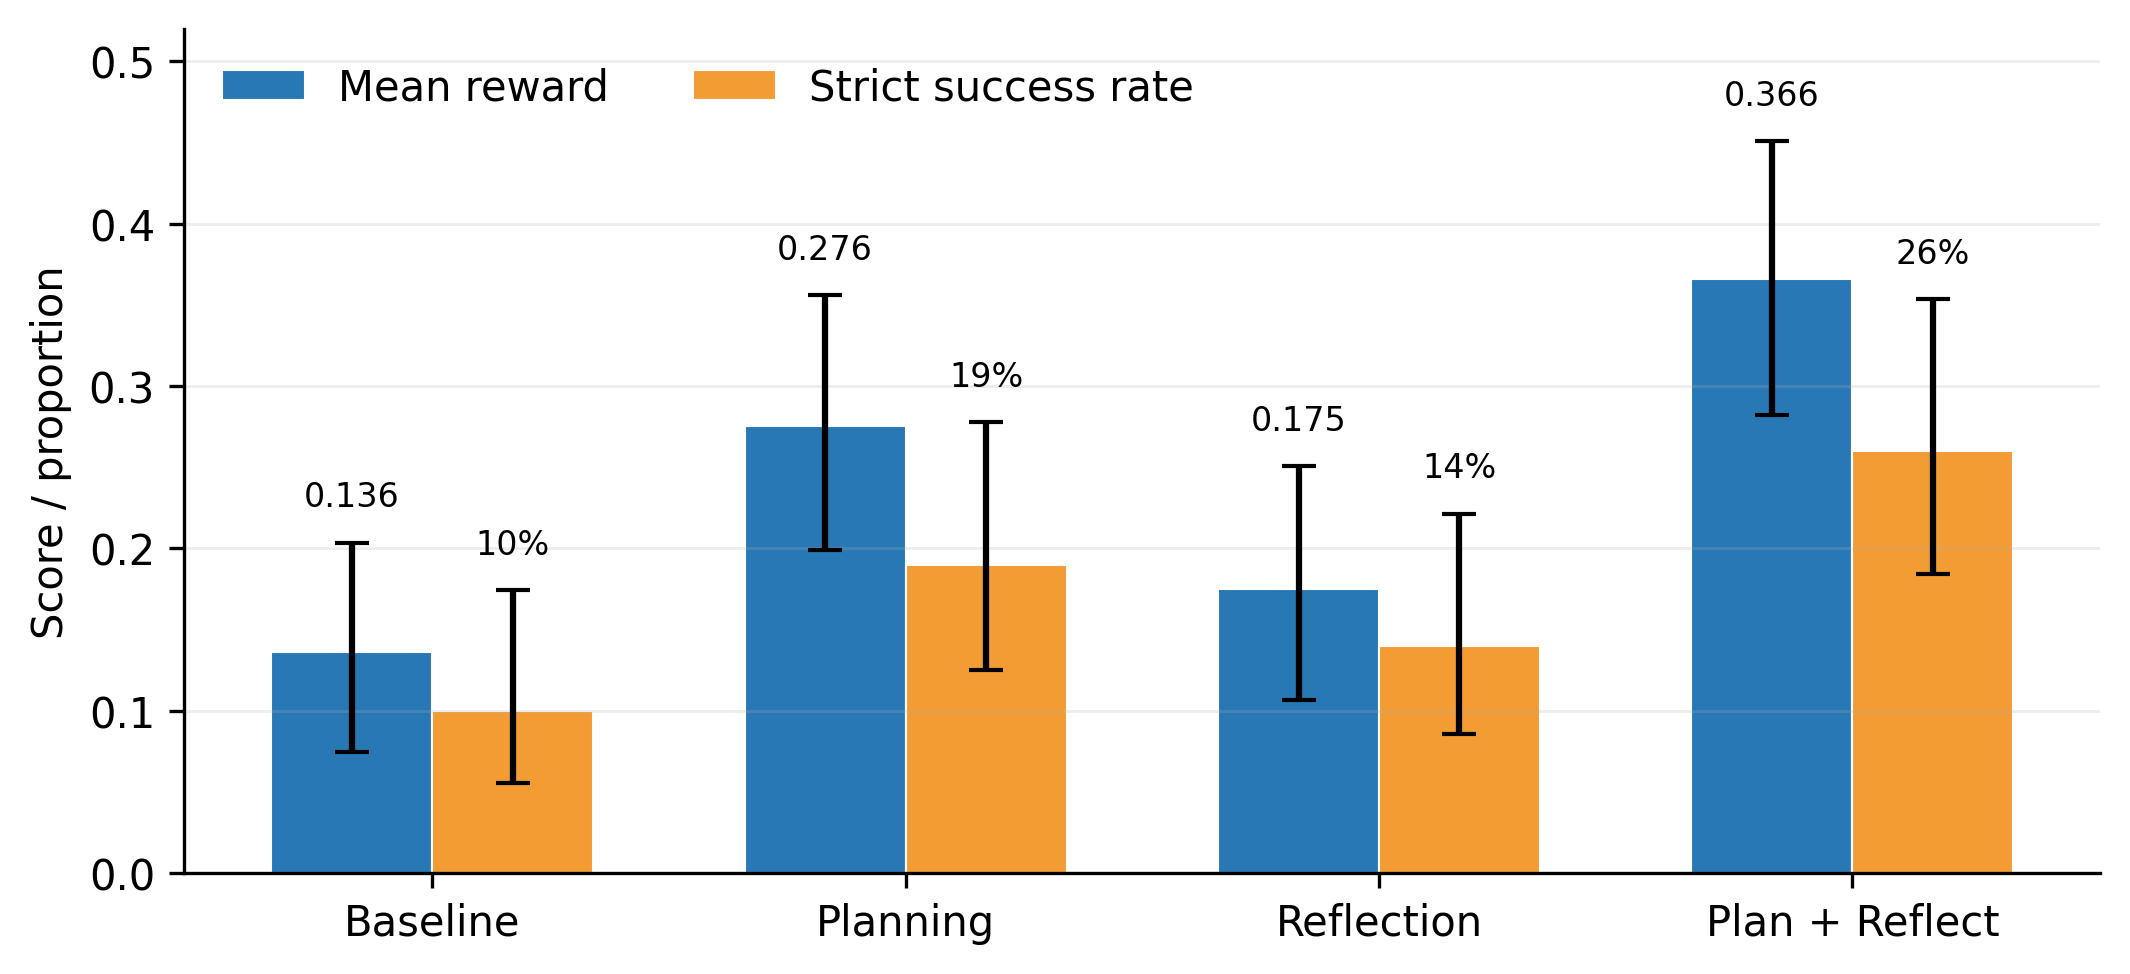
\includegraphics[width=\linewidth]{figures/performance.png}
  \caption{Mean reward and strict success with 95\% confidence intervals.}
  \label{fig:performance}
\end{minipage}\hfill
\begin{minipage}{0.49\textwidth}
  \centering
  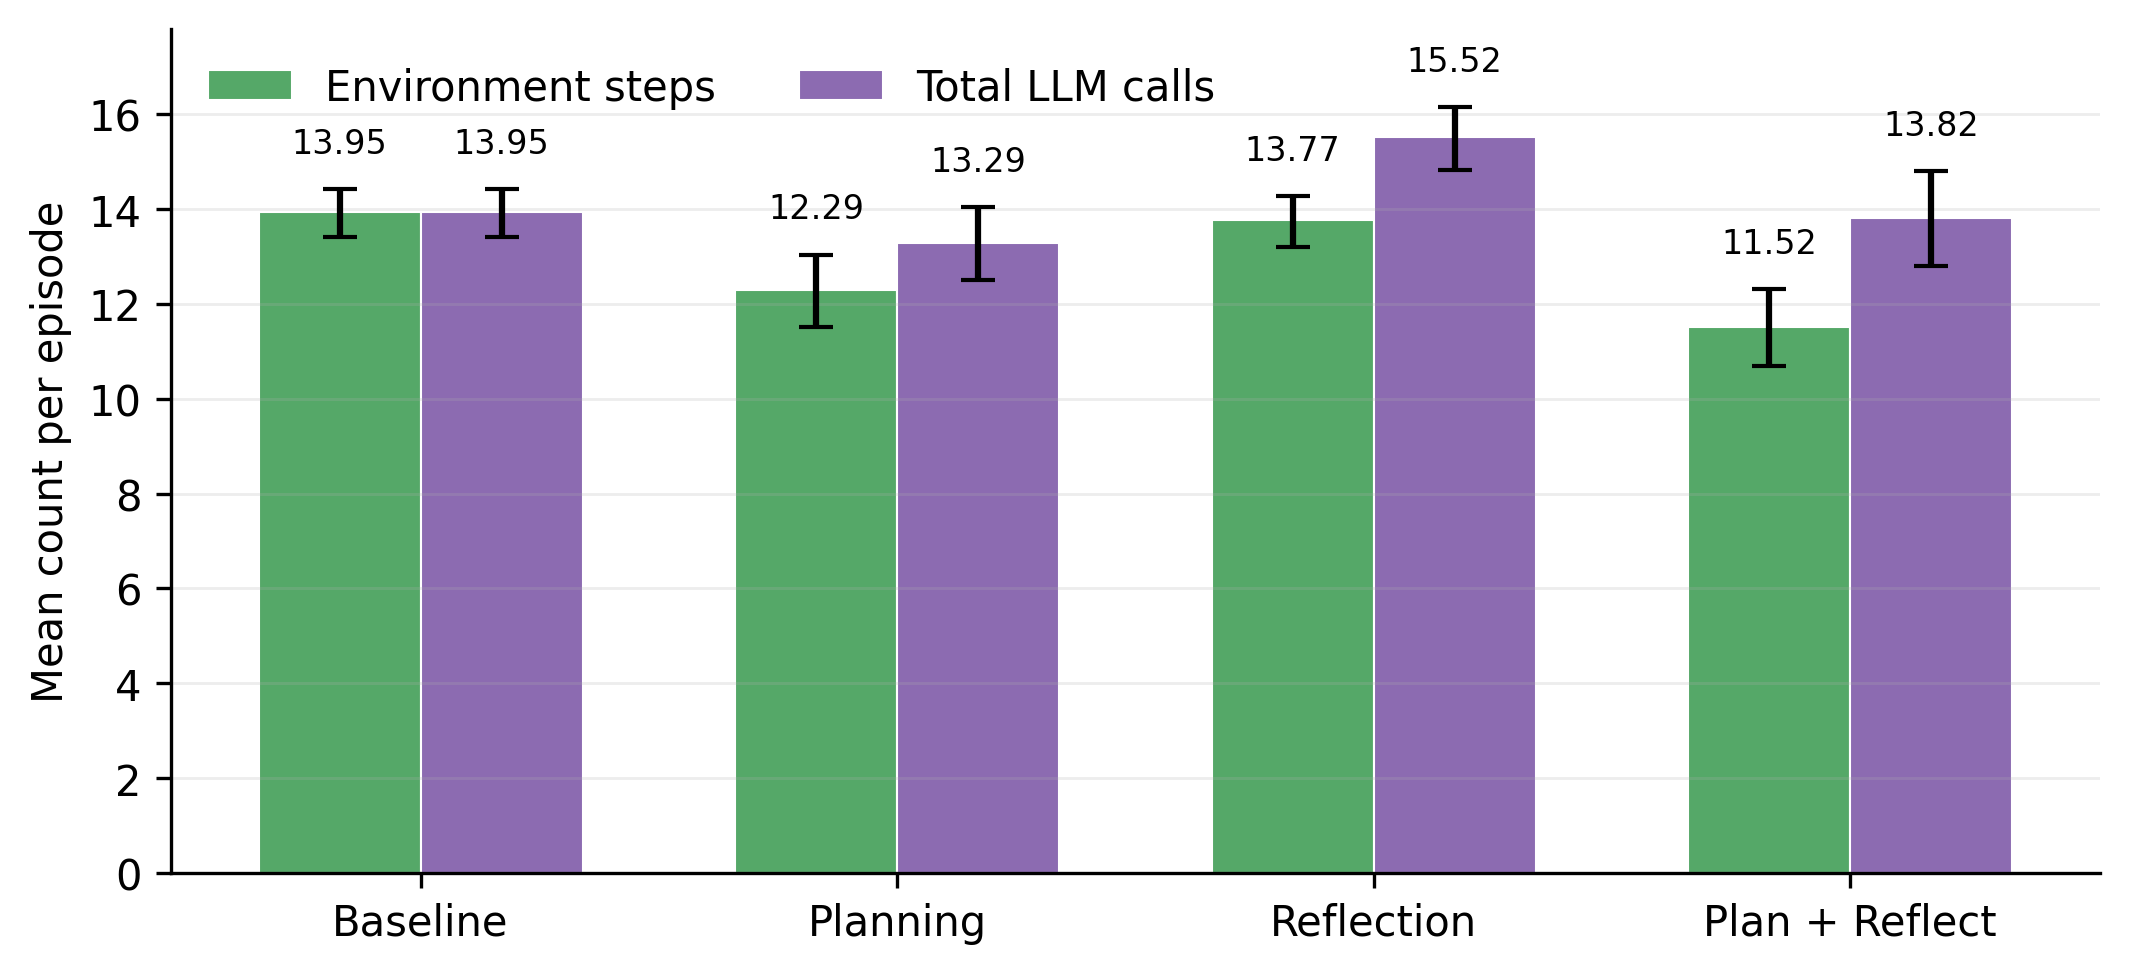
\includegraphics[width=\linewidth]{figures/efficiency.png}
  \caption{Environment steps and total model calls per episode.}
  \label{fig:efficiency}
\end{minipage}
\end{figure*}

\subsection{Paired comparisons}

\begin{table*}[t]
\centering
\caption{Paired comparisons against Baseline. Reward and success $p$-values are Holm-corrected within their respective three-comparison families. ``B-only/T-only'' counts discordant strict successes.}
\label{tab:paired}
\small
\setlength{\tabcolsep}{5pt}
\resizebox{\textwidth}{!}{%
\begin{tabular}{lccccc}
\toprule
Comparison & Reward difference (95\% CI) & Reward $p$ & B-only/T-only & McNemar $p$ & LLM-call difference \\
\midrule
Planning vs. Baseline & $+0.139$ $[+0.047,+0.231]$ & 0.0074 & 5/14 & 0.1271 & $-0.66$ \\
Reflection vs. Baseline & $+0.039$ $[-0.035,+0.115]$ & 0.3320 & 4/8 & 0.3877 & $+1.57$ \\
\ours\ vs. Baseline & $+0.230$ $[+0.136,+0.327]$ & $<0.0001$ & 4/20 & 0.0046 & $-0.13$ \\
\bottomrule
\end{tabular}
}
\end{table*}

The paired analysis in Table~\ref{tab:paired} strengthens the aggregate result. Planning and \ours have reward-difference intervals entirely above zero. Planning's strict-success improvement is directionally favorable but not significant after multiplicity correction. In contrast, \ours has 20 tasks that only it solves versus four solved only by Baseline, producing a corrected exact McNemar $p$-value of 0.0046. Reflection alone does not provide conclusive evidence on either primary metric.

Although planning and reflection add auxiliary requests, successful early termination offsets much of this cost in total call count. Planning averages fewer total calls than Baseline, and \ours is nearly equal to Baseline. This does not imply equal runtime: mean episode latency is 67.7 seconds for Baseline, 89.7 for Planning, 72.8 for Reflection, and 115.6 for \ours. Auxiliary calls produce longer outputs, and web/API response time varies despite interleaving.

\subsection{Factorial effects}

The reward-scale planning main effect is $+0.165$ (95\% CI $[+0.091,+0.238]$), averaging its effect with and without reflection. The reflection main effect is $+0.065$ ($[+0.010,+0.120]$). The planning-by-reflection interaction is $+0.051$ ($[-0.059,+0.162]$). Thus, the full method is empirically strongest, but the current sample does not establish a super-additive interaction. This distinction prevents the descriptive superiority of the combination from being overstated as statistical synergy.

\section{Behavioral Analysis}

\subsection{Failure indicators}

The dominant failure mode is exhaustion of the 15-step budget. Baseline reaches this limit on 84 tasks, frequently because the model emits repeated reasoning without a state-changing action. Planning reduces this rate to 63\%; the combined method reduces it further to 53\%. Reflection-only remains high at 80\%, indicating that a verbal diagnosis does not guarantee that the next decoded action follows it.

Planning has the highest invalid-action rate (10.8\%). This is partly a byproduct of attempting more varied navigation and verification steps rather than remaining in a reasoning loop. Reflection outputs also have formatting failures: 16 malformed auxiliary responses occur in the Reflection condition, compared with three for \ours. The plan context may stabilize later critique formatting, but this observation is correlational and the experiment was not designed to isolate format compliance mechanisms.

Across the 100 tasks, no method achieves strict success on 66 tasks. The remaining success patterns are diverse: seven tasks are solved only by \ours, six by Planning and \ours, five by Planning, Reflection, and \ours, and several by other combinations. This heterogeneity motivates paired evaluation; a single aggregate success rate hides large task-level differences.

\subsection{Representative trajectories}

\begin{table*}[t]
\centering
\caption{Condensed qualitative cases. These examples illustrate observed mechanisms but do not replace the paired aggregate analysis.}
\label{tab:cases}
\small
\setlength{\tabcolsep}{4pt}
\begin{tabular}{lP{0.18\textwidth}P{0.28\textwidth}P{0.30\textwidth}}
\toprule
Task & Instruction & Baseline behavior & Enhanced behavior \\
\midrule
\texttt{fixed\_17} & MN4 foundation for sensitive skin under \$40 & Repeated an invalid navigation hypothesis and exhausted 15 steps with reward 0. & Reflection diagnosed the invalid back-navigation action, revised the query strategy, inspected the closest result, selected option \texttt{mn4}, and purchased correctly in 12 steps. \\
\texttt{fixed\_49} & Engineered-wood end table under \$150 & Baseline repeated a search intention without executing search; Planning found a suitable product but attempted purchase from the wrong page; Reflection-only repeated thoughts. & \ours tracked material, category, and price constraints, used reflection after malformed and invalid actions, returned to the item page, and achieved reward 1 in 11 steps. \\
\bottomrule
\end{tabular}
\end{table*}

Task \texttt{fixed\_17} illustrates the intended benefit of triggered recovery: the critique points to concrete evidence from the invalid action and proposes a valid state-changing alternative. Task \texttt{fixed\_49} shows why planning and reflection are complementary at the trajectory level. The plan identifies what must be verified; reflection repairs execution after the agent violates the page-state constraints. However, these cases also expose a limitation: model-generated reflection is advice to the same fallible policy, not a hard controller, so compliance is not guaranteed.

\section{Discussion}

The results answer the three research questions. First, planning improves reward and reduces budget exhaustion, supporting the hypothesis that explicit constraint tracking and verification are valuable in WebShop. Second, reflection can recover individual failures, but its standalone average effect is uncertain. Third, combining the components gives the best observed performance and a robust advantage over Baseline, yet the interaction confidence interval crosses zero. The evidence therefore supports using both components, while favoring an additive interpretation over a claim of proven synergy.

An important practical result is that auxiliary reasoning should be evaluated jointly with environment efficiency. A method may spend an additional planning call yet reduce the total number of action calls by finishing earlier. Conversely, token and wall-clock costs remain higher even when total call counts are similar. Reporting only success or only model calls would give an incomplete view.

The study also suggests possible improvements. Reflection could be coupled to constrained action decoding so that a revised strategy must lead to an admissible action type. Page-state information could be represented explicitly rather than inferred from prose. Finally, a learned or rule-based trigger might allocate reflection calls only when their expected value exceeds their latency cost.

\section{Limitations and Responsible Use}

The experiment uses one model backend, one prompt family, one run per method-task pair, and 100 held-out tasks. Results may change with different model sizes, demonstrations, or decoding systems. WebShop is realistic but still simulated; performance does not establish safety on live commerce websites. The one-page search restriction and 15-step budget intentionally simplify the environment but also create failures that a less restricted browser agent might avoid. API and environment latency remain noisy despite cyclic interleaving. Finally, the analysis tests prompt-time scaffolding, not learning: no parameters are updated and no cross-episode memory is used.

No real purchases, personal data, or human subjects are involved. Nevertheless, deploying a similar agent on a live website would require confirmation before purchases, protection of user data, robust handling of price changes, and safeguards against misleading product content. Model-generated reasoning and reflection should not be treated as guaranteed faithful explanations.

\section{Conclusion}

This work presents a reproducible ablation of planning and triggered reflection for ReAct-style WebShop agents. Explicit planning is the stronger individual intervention, while reflection alone is variable. Their combination achieves the highest mean reward and strict success, with statistically reliable paired gains over Baseline and substantially fewer step-limit terminations. At the same time, higher latency, remaining hard tasks, and a non-significant interaction estimate temper the conclusion. Lightweight deliberation is useful, but reliable web agents also need mechanisms that translate plans and critiques into valid state-aware actions.

\section*{Reproducibility Statement}

The accompanying code separates the four agents, shared environment adapter, prompts, configurations, runner, and statistical analysis. Formal configurations record the model, decoding settings, WebShop Git commit \texttt{64fa2a5c15c7daa698b9ac93f5bb5437b634c9bd}, full-dataset version \texttt{YWZBrandon/webshop-data@ce990fff5aee388db2706f07820c578ab68e0453}, prompt versions, and environment patch version. Raw JSONL trajectories contain actions, observations, rewards, trigger events, token counts, and latency. The analysis script verifies 100 unique paired tasks per method before regenerating all reported tables, confidence intervals, tests, and figures with a fixed seed.

\bibliographystyle{plainnat}
\bibliography{references}

\appendix

\section{Additional Efficiency Results}

\begin{table}[h]
\centering
\caption{Additional per-episode resource metrics.}
\label{tab:resources}
\small
\begin{tabular}{lrrrr}
\toprule
Method & Input tok. & Output tok. & LLM sec. & Episode sec. \\
\midrule
Baseline & 13,729 & 481 & 13.81 & 67.72 \\
Planning & 14,051 & 490 & 14.60 & 89.67 \\
Reflection & 15,852 & 640 & 16.92 & 72.79 \\
\ours & 15,323 & 542 & 16.89 & 115.57 \\
\bottomrule
\end{tabular}
\end{table}

\section{Implementation Details}

Planning is called exactly once per episode when enabled. Reflection is capped at two calls; the observed averages are 1.75 for Reflection-only and 1.30 for \ours. The reflection history contains at most five recent steps. Shared HTTP requests use two retries, and formal WebShop requests use a 60-second timeout. Environment errors are excluded from method outcomes and retried after service recovery; the final 400-record dataset contains zero environment-error rows. Auxiliary output formatting is validated and logged but not manually repaired.

\end{document}
